\documentclass[tikz, border=10pt]{standalone}
\usepackage[utf8]{inputenc}
\usetikzlibrary{shapes.geometric, arrows.meta, positioning, fit, backgrounds, calc, chains, scopes}

\definecolor{colorInit}{HTML}{FFF9E6}
\definecolor{colorLoop}{HTML}{E6F3FF}
\definecolor{colorDecision}{HTML}{FFCC00}
\definecolor{colorEnd}{HTML}{D1D5DB}

\begin{document}

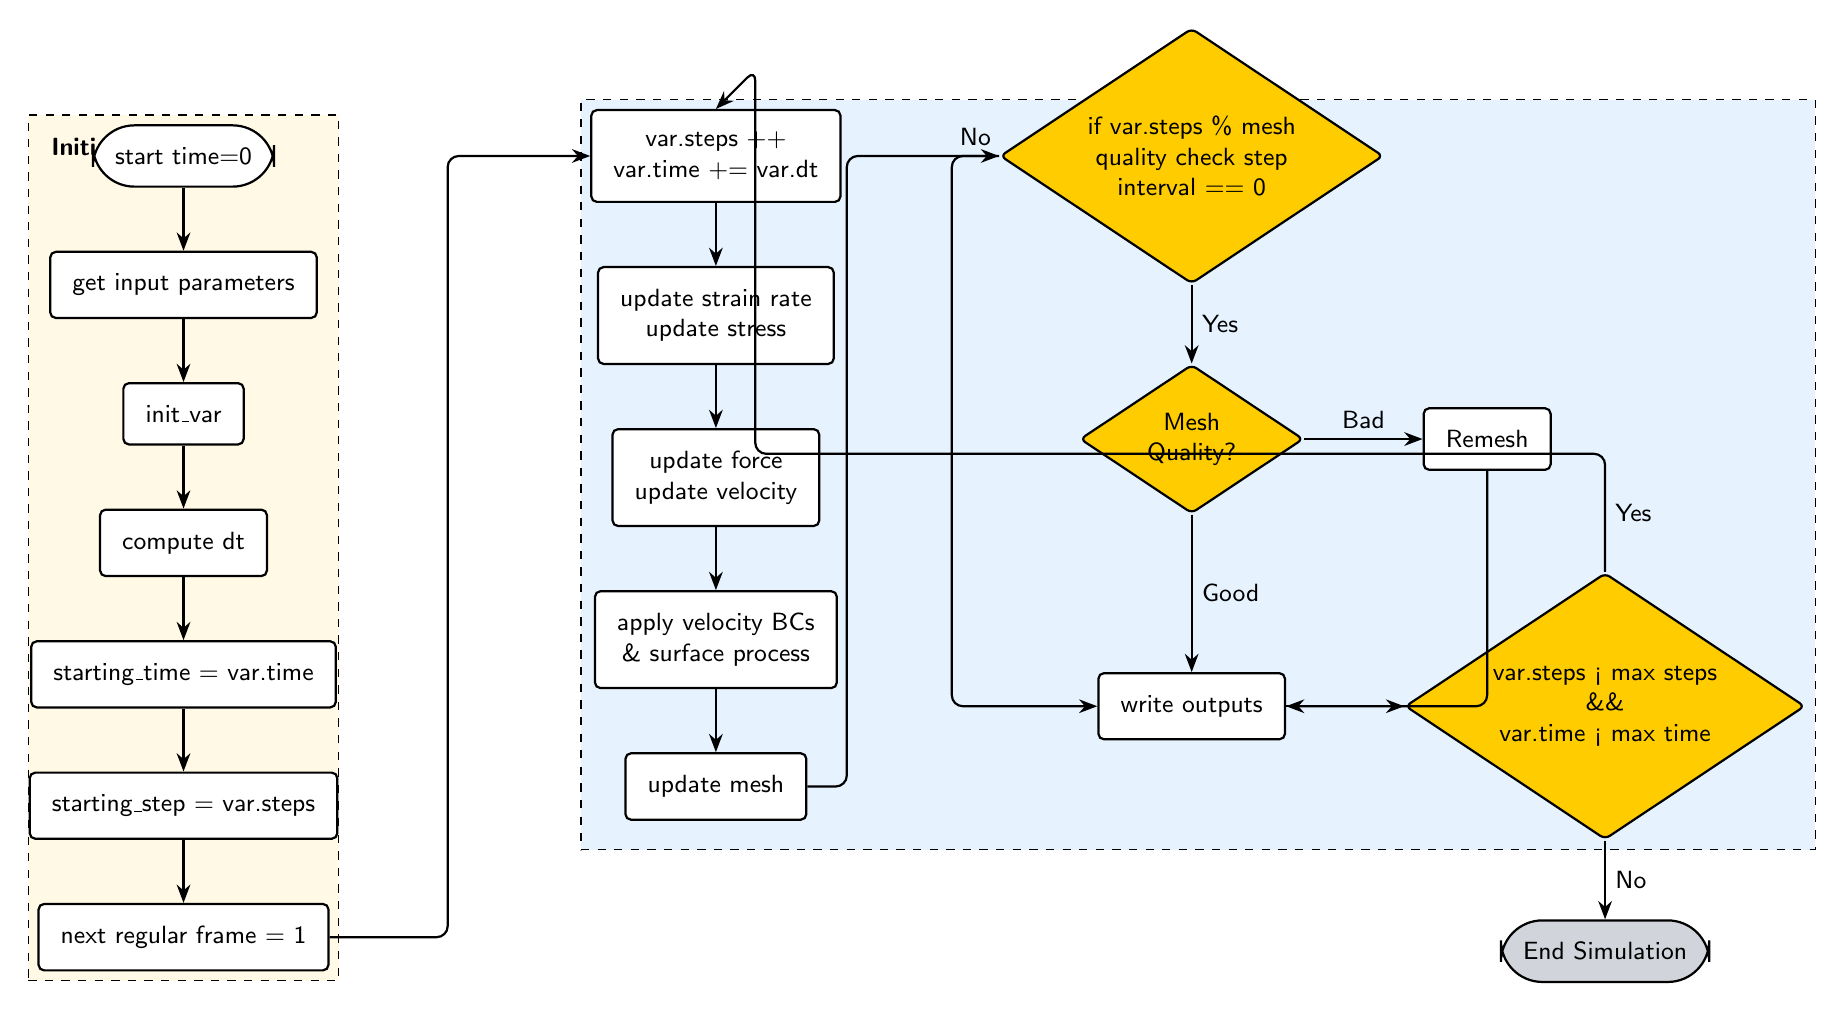
\begin{tikzpicture}[
    node distance=0.8cm and 1.5cm,
    font=\sffamily\small,
    base/.style = {
        draw, 
        align=center, 
        minimum height=3.5ex,
        inner sep=8pt,
        rounded corners=2pt,
        thick
    },
    startstop/.style = {
        base, 
        shape=rectangle, 
        rounded corners=15pt, 
        fill=white
    },
    process/.style = {
        base, 
        shape=rectangle,
        fill=white
    },
    decision/.style = {
        base, 
        shape=diamond, 
        aspect=1.5,
        fill=colorDecision,
        inner sep=4pt
    },
    endnode/.style = {
        base,
        shape=rectangle,
        rounded corners=15pt,
        fill=colorEnd
    },
    arrow/.style = {
        thick, 
        ->, 
        >=Stealth,
        rounded corners
    }
]

    % --- Initialization Group ---
    \begin{scope}[start chain=init going below]
        \node [startstop, on chain] (start_time) {start time=0};
        \node [process, on chain] (get_params) {get input parameters};
        \node [process, on chain] (init_var) {init\_var};
        \node [process, on chain] (compute_dt) {compute dt};
        \node [process, on chain] (starting_time) {starting\_time = var.time};
        \node [process, on chain] (starting_step) {starting\_step = var.steps};
        \node [process, on chain] (next_frame) {next regular frame = 1};
    \end{scope}

    % --- Main Loop Section ---
    % Position var_update to the right of Initialization group
    % We align it with the top of the initialization chain (start_time)
    \node [process, right=4cm of start_time] (var_update) {var.steps ++ \\ var.time += var.dt};

    \begin{scope}[start chain=loop going below]
        % We manually chain from var_update
        \node [process, below=of var_update] (strain_stress) {update strain rate \\ update stress};
        \node [process, below=of strain_stress] (force_vel) {update force \\ update velocity};
        \node [process, below=of force_vel] (velocity_bc) {apply velocity BCs \\ \& surface process};
        \node [process, below=of velocity_bc] (update_mesh) {update mesh};
    \end{scope}

    % Move mesh logic to the right of var_update column
    % Let's align it with var_update vertically (top) or relative to update_mesh?
    % "Move the decision node... to the right of the var_update node."
    % The user likely means the *block* starting with mesh_check_logic should be to the right of the main vertical column.
    
    % Positioning mesh_check_logic to the right of "update_mesh" (the bottom of the first column) or "var_update"?
    % If I move it to the right of var_update, it will be very high up. 
    % But the connection is update_mesh -> mesh_check_logic.
    % If I move it right of 'var_update', the arrow goes from bottom of col 1 to top of col 2.
    
    \node [decision, right=2cm of var_update] (mesh_check_logic) {if var.steps \% mesh \\ quality check step \\ interval == 0};

    % --- Side Branch for Mesh Quality ---
    % Place 'mesh_quality_dec' below 'mesh_check_logic' since we are now in a new column on the right
    \node [decision, below=1cm of mesh_check_logic] (mesh_quality_dec) {Mesh \\ Quality?};
    
    % Place 'remesh' right of 'mesh_quality_dec' to save vertical space or keep below?
    % Let's keep it below for flow consistency or right?
    % If below:
    \node [process, right=1.5cm of mesh_quality_dec] (remesh) {Remesh};

    % --- Rejoin Point ---
    % 'write_outputs' logic needs to be handled.
    % Path 1: mesh_check_logic (No) -> write_outputs
    % Path 2: mesh_quality_dec (Good) -> write_outputs
    % Path 3: remesh -> write_outputs
    
    % detailed placement:
    % write_outputs can be below mesh_quality_dec
    \node [process, below=2cm of mesh_quality_dec] (write_outputs) {write outputs};

    % --- Final Check ---
    % Move sim_check to the right of write_outputs
    \node [decision, right=1.5cm of write_outputs] (sim_check) {var.steps < max steps \\ \&\& \\ var.time < max time};
    
    \node [endnode, below=1cm of sim_check] (end_sim) {End Simulation};

    % --- Backgrounds ---
    \begin{scope}[on background layer]
        % Initialization Background
        \node [fit=(start_time)(next_frame), fill=colorInit, draw, dashed, label={[anchor=north west, shift={(5pt,-5pt)}]north west:\textbf{Initialization}}] (init_bg) {};
        
        % Main Loop Background
        % It includes var_update down to sim_check, covering the width of remesh too
        \node [fit=(var_update)(sim_check)(remesh)(mesh_quality_dec), fill=colorLoop, draw, dashed, label={[anchor=north west, shift={(5pt,-5pt)}]north west:\textbf{Main Loop}}] (loop_bg) {};
    \end{scope}

    % --- Connections ---
    
    % Initialization chain
    \draw [arrow] (start_time) -- (get_params);
    \draw [arrow] (get_params) -- (init_var);
    \draw [arrow] (init_var) -- (compute_dt);
    \draw [arrow] (compute_dt) -- (starting_time);
    \draw [arrow] (starting_time) -- (starting_step);
    \draw [arrow] (starting_step) -- (next_frame);
    
    % Into loop
    \draw [arrow] (next_frame.east) -- ++(1.5cm,0) |- (var_update.west);
    
    % Loop chain vertical
    \draw [arrow] (var_update) -- (strain_stress);
    \draw [arrow] (strain_stress) -- (force_vel);
    \draw [arrow] (force_vel) -- (velocity_bc);
    \draw [arrow] (velocity_bc) -- (update_mesh);
    % Connection from bottom of col 1 to top of col 2 (mesh_check_logic)
    \draw [arrow] (update_mesh.east) -- ++(0.5cm,0) |- (mesh_check_logic.west);

    % Mesh Check Logic
    \draw [arrow] (mesh_check_logic) -- node[right] {Yes} (mesh_quality_dec);
    % No path -> write_outputs. write_outputs is below mesh_quality_dec.
    % We need to go around mesh_quality_dec.
    \draw [arrow] (mesh_check_logic.west) -- node[above] {No} ++(-0.6cm,0) |- (write_outputs.west);

    % Mesh Quality Logic
    \draw [arrow] (mesh_quality_dec) -- node[above] {Bad} (remesh);
    % Good path: Direct down to write_outputs
    \draw [arrow] (mesh_quality_dec) -- node[right] {Good} (write_outputs);
    
    % Remesh -> write_outputs
    \draw [arrow] (remesh) |- (write_outputs);
    
    % Write Outputs -> Sim Check
    \draw [arrow] (write_outputs) -- (sim_check);

    % Sim Check Logic
    \draw [arrow] (sim_check) -- node[right] {No} (end_sim);
    
    % The Big Loop Back (Yes)
    % From sim_check back to var_update.
    % sim_check is far right. var_update is left. mesh_check_logic is in between.
    % We route Up from sim_check, go above mesh_check_logic, and drop into var_update.
    \draw [arrow] (sim_check.north) -- node[right] {Yes} ++(0, 1.5cm) coordinate(top_turn) 
        -| ($(var_update.north) + (0.5cm, 0.5cm)$) -- (var_update.north);

\end{tikzpicture}

\end{document}
